\documentstyle[12pt,epsfig]{article}
\begin{document}

\section{Ecotox and bioenergetics modelling within IBMlib} 

This document is an addition to documentation for module IBM (implementation IBMlib at DTU Aqua)
submitted as deliverable 2.11 for EU FP7 MEECE. 

\subsection{Generic bioenergetics} 

generic\_bioenergetics is an embedded frame work within IBMlib to 
\begin{enumerate}
  \item make flexible multi stage modelling, based on independent sub stages
  \item model growth energy budgets for early life stages
  \item provide a starting point for derivative models, e.g. ecotox impact modelling
\end{enumerate} 
generic\_bioenergetics delivers the particle\_state interface for IBMlib.
The main idea is to localize species specific properties in particular modules
to ensure portability to new species.
generic\_bioenergetics focuses on early life stages where the natural internal units 
are $\mu$g for weight, mm for length and seconds for time.
Currently, internal classes within generic\_bioenergetics have public scope (for the time being)

\subsection{Multi stage modelling} 

Multi stage modelling is handled by a light weight bundling module that 
combines independent stages described by classes in other modules. The multi stage module
offers a class has independent stage class instances as components. A multi stage instance
manages which stage is currently active and handles overall attributes, like the survival chance
of the organism, place and time of origin. The multi stage class interacts with independent stages
via the particle\_sub\_state interface described below

\subsubsection{Stage components} 

  Each ontogenetic stage is implemented in a module providing a particle\_sub\_state interface.
  These implementations may be species specific or generic, e.g. implementing a behavioral model 
 (like optimal feeding larvae, optimal\_forager.f).
  Currently, the multi stage class expects three sub classes to be present at compilation time
  (by selecting appropriate options in the make file)

  \begin{itemize}
  \item module feeding\_larval\_stage   
  \item module yolksac\_larval\_stage                    
  \item module released\_egg\_stage 
  \end{itemize}

  Stage classes may also by themselves provide the full particle\_state interface in parallel
  with particle\_sub\_state interface. To use this, a module name conversion dummy should
  be used. Currently this is only available for the implementation optimal\_forager.f 
  implementating module feeding\_larval\_stage   


% ----------------------------------------------------------------------------
\begin{figure}[p]   % [tbhp]
\begin{center}                                                 
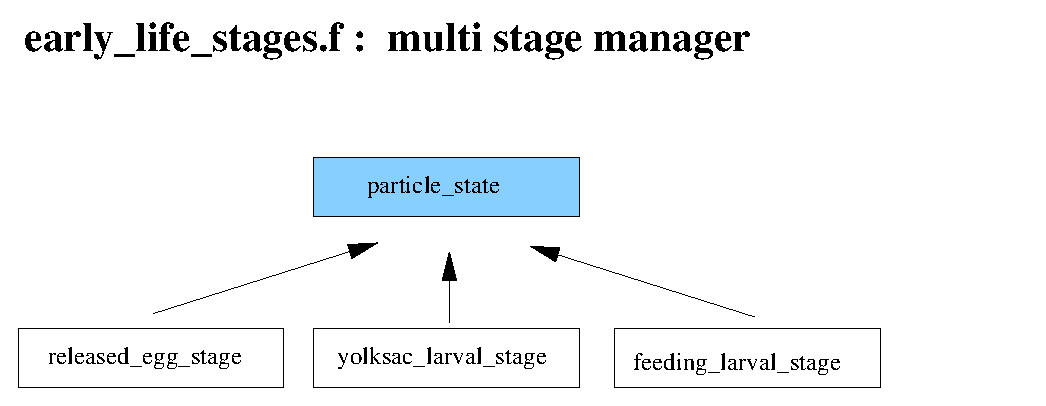
\epsfig{file=early_life_stages_light.eps,width=120mm,angle=0,clip=}     
\end{center}                                                    
\caption{Inheritance diagram for multi stage manager}
\label{multistagemanager:fig}
\end{figure}
% ----------------------------------------------------------------------------


\subsubsection{particle\_sub\_state interface} 

The particle\_sub\_state interface is implemented by the decorator modules.
If X designates the stage (e.g. X=feeding\_larvae) then the particle\_sub\_state interface has the following 
components:
\begin{itemize}
  \item type X. This class is embedded in the multi stage class representing a multi staged organism.

 \item subroutine update\_particle\_state\_X(state, space, dt, mortality\_rate, die, next)  \newline
type(X), intent(inout)     :: state  \newline
type(spatial\_attributes), intent(inout) :: space  \newline
real,intent(in)                         :: dt ! in seconds  \newline
real,intent(out)                        :: mortality\_rate  \newline
logical,intent(out)                     :: die, next  \newline


 \item subroutine init\_state\_attributes\_X(state, space, time\_dir,  initdata)  \newline
type(X),intent(out)       :: state  \newline
type(spatial\_attributes),intent(inout) :: space  \newline
real,intent(in)                        :: time\_dir   \newline           
character*(*),intent(in)               :: initdata  \newline


 \item subroutine get\_active\_velocity\_X(state, space, v\_active)  \newline
type(X), intent(in)     :: state  \newline
type(spatial\_attributes), intent(in) :: space  \newline      
real, intent(out)                    :: v\_active(:) ! meter/second  \newline


\end{itemize}

Note that the particle\_sub\_state interface is rather similar to the particle\_state interface, but that
update\_particle\_state\_X features extra output parameters mortality\_rate, die, next. These
parameters are needed by the multi stage manager to make stage transitions and manage overall
properties, like survival of the organism. The particle\_sub\_state interface for a particular stage will only
be applied if the stage is currently active.


\subsection{Growth energy budgets for early life stages} 

module feeding\_larval\_stage  in the implementation  optimal\_forager.f implements 
foraging based on optimal foraging theory (Charnov 1975). Diet switching is controlled completely by 
size-based processes in capture\_sucess, handling\_time, search\_volume provided by module larval\_properties. 
The continuous food spectrum is size based as provided by module prey\_community with prey\_spectrum\_density.
  
optimal\_forager.f can determine the maximal food intake (corresponding to the optimal diet) from a continuous food spectrum 
either by on-the-fly diet optimization or from a pretabulated data base of optimal diets for a reference database
set in the input file. The latter mode is for production runs, to avoid optimization for each organism in each 
time step. If the reference database is set appropriately, the results should be similar, to within numerical accuracy.
To set reference database, see input parameters for module feeding\_larval\_stage below.

\subsection{Ecotox representation} 

Parameterization of copper impact on early life stages is based on experiments of Tanja St. John 
 within EU FP7 MEECE. Experiments address egg+yolksac of sprat and the paragraph below describes
how results of experiments are implemented within IBMlib

Parameterization covers
\begin{enumerate}
   \item The decrease in egg survival (hatch fraction)
   \item The decrease in larval hatch length
\end{enumerate}
including temperature dependence. Experiments only cover egg+yolksac stages
and only addresses egg survival and hatch length (no other impact mechanisms).
%% ===========================================================================
\subsubsection{Egg survival} 

The decrease in egg survival (hatch fraction) in the meta parameterization is represented as 
\begin{eqnarray*}
          S(c,T) & = & S_0(T) exp(- c / K_2(T))  \\
          S_0(T)  & = & A_0*(1 - exp(-A_1*(T-A_2)))\\
          K_2     & = & 50 {\ \rm yg/l} \\
	  A_0     & = & 0.231794 \\
          A_1     & = & 0.286788 \\
          A_2     & = & 5.68092  \\
\end{eqnarray*}
with $T$ as $^\circ$C and copper concentration $c$ as yg/l.
Copper-temperature interaction are skipped, because variability of $K_2$(T)
from experiments seem spurious, and $K_2$ has been fixed to $K_2  = 50 $yg/l.

This corresponds to an instantaneous mortality $Z(c,T)$ formulation as 
\begin{equation}
           S(c,T) =  exp( -Z(c,T)/g(c,T) ) \nonumber
\end{equation}
where $g(c,T)$ is the egg development rate (expressed as fraction per time) with the
implicit assumption that egg loss is uniformly distributed over egg development phase
(this assumption only matters, if dynamics within egg development phase is considered).
Egg survival fraction as function of copper concentration is plotted in Fig. \ref{survANDhlen}(left)
$g(c,T)$ is parameterized following Deawel et al. (2008).
%% ===========================================================================
\subsubsection{Decrease in larval hatch length} 

The decrease in larval hatch length $L_h$ in the meta parameterization is represented as 
\begin{eqnarray*}
 L_h(c,T) = L_0 exp(- c / K_1(T)) + L_{\inf}  \\
 L_0      = 7 {\ \rm mm} \\
 L_{\inf}  = 5 {\ \rm mm} \\
 K_1(T)   = 0.00049 * T^{5.95} {\ \rm yg/l} \\
\end{eqnarray*}
with $T$ as $^\circ$C and copper concentration $c$ as yg/l.
Larval hatch length as function of copper concentration is plotted in Fig. \ref{survANDhlen}(right)
% ----------------------------------------------------------------------------
\begin{figure}[p]   % [tbhp]
\begin{center}                                                 
\epsfig{file=S.eps,width=60mm,angle=0,clip=}    
\epsfig{file=L.eps,width=60mm,angle=0,clip=}    
\end{center}                                                    
\caption{Left: egg survival fraction as function of copper concentration for T = 6 and 12 $^\circ$C.
Right: larval hatch length as function of copper concentration for T = 6 and 12 $^\circ$C.}
\label{survANDhlen}
\end{figure}
% ----------------------------------------------------------------------------

The implementation above is committed as IBMlib SVN revision 415.



\section{Module listing } 

%------------------------------------------------------------------------------------------------------------------
\subsection{Decorators} 
%------------------------------------------------------------------------------------------------------------------

\subsubsection{module feeding\_larval\_stage}                                     
implementation : optimal\_forager.f.
particle\_state interface/sub interface for feeding larval stage  
This version applies optimal foraging theory in relation to a size spectrum, based
on larval performance capture\_sucess/handling\_time/search\_volume
prescribed in module larval\_properties 

\begin{verbatim}
type feeding_larvae
      private
         type(larval_physiology) :: larvstate         ! defined in module larval_properties 
      end type
      public :: feeding_larvae ! make type state_attributes visible outside

 type state_attributes



      public :: init_particle_state  ! module operator
      public :: close_particle_state ! module operator
      public :: init_state_attributes
      public :: get_active_velocity
      public :: update_particle_state
      public :: delete_state_attributes 
      public :: write_state_attributes
      public :: get_particle_version
      public :: get_property         ! currently void
      public :: get_metadata_state   ! currently void

      public :: init_feeding_larval_stage
      public :: close_feeding_larval_stage
      public :: init_state_attributes_FL
      public :: get_active_velocity_FL
      public :: update_particle_state_FL
      public :: delete_state_attributes_FL
\end{verbatim}

Input parameters (for simulation file):\newline
\begin{itemize}
  \item ingestion\_integral\_sampling (integer). Diet integrals over
        size spectra are calculated using numerical integrals. This parameter
        tells how many sampling points are used for numerical integrals.  
  \item precalc\_ingestion\_DB (logical). Whether to generate a database of
        maximal intake (.true.) or calculate  maximal intake on the fly for each larvae in 
        each time step (.false.)
        If precalc\_ingestion\_DB is .true. then the following parameters
        specifying the reference database is generated
        \begin{itemize}
          \item larval\_length\_grid\_min (mm) feeding larval range, start
          \item larval\_length\_grid\_max (mm) feeding larval range, end
          \item larval\_length\_grid\_points (integer) sampling of larval range.
          \item logZ\_grid\_min (log(kg DW/m3)) Zooplankton range, start
          \item logZ\_grid\_max (log(kg DW/m3)) Zooplankton range, end
          \item logZ\_grid\_points (integer) sampling of zooplankton range.
          \item julian\_day\_grid\_points (integer) sampling of seasonal cycle
  \end{itemize}
\end{itemize}

%--------------------------------------------------------------------------------------
\subsubsection{module yolksac\_larval\_stage}                     implementation : yolksac\_larval\_stage.f

particle\_state sub interface for yolksac\_larval\_stage for
multi stage manager. Species specific properties comes from 
module yolksac\_properties     

\begin{verbatim}
type yolksac_larvae
      private
         real :: completion   ! 0 < completion < 1. Hatch at 1
      end type
      public :: yolksac_larvae ! make type state_attributes visible outside


c.....Particle sub state interface: (for multi stage manager)
      public :: init_yolksac_larval_stage  ! module operator
      public :: close_yolksac_larval_stage ! module operator
      public :: init_state_attributes_YL
      public :: get_active_velocity_YL
      public :: update_particle_state_YL
      public :: delete_state_attributes_YL
\end{verbatim}


%--------------------------------------------------------------------------------------
\subsubsection{module released\_egg\_stage}                        
implementation : released\_egg\_stage.f
particle\_state sub interface for released\_egg\_stage for
multi stage manager. Species specific properties comes from 
module yolksac\_properties     


\begin{verbatim}
type released_egg
      private
         real :: completion   ! 0 < completion < 1. Hatch at 1
      end type
      public :: released_egg ! make type state_attributes visible outside


c.....Particle sub state interface: (for multi stage manager)
      public :: init_released_egg_stage  ! module operator
      public :: close_released_egg_stage ! module operator
      public :: init_state_attributes_egg
      public :: get_active_velocity_egg
      public :: update_particle_state_egg
      public :: delete_state_attributes_egg

\end{verbatim}

%--------------------------------------------------------------------------------------
\subsubsection{module particle\_state}                             
implementation : early\_life\_stages.f
multi stage manager implementing particle\_state interface 
from merging sub interfaces

released\_egg\_stage + yolksac\_larval\_stage + feeding\_larval\_stage  



\end{document}
